% ===== classification-evaluation =====
\section*{Evaluating Classifiers \& Multiclass}
% ---- CS189 scope checklist: must include ([x] = already covered) ----
% Source: Lectures 4, 9; reference sheet p.7
% [ ] Confusion matrix: TP, TN, FP, FN
% [ ] Accuracy, precision, recall (= TPR), FPR
% [ ] F1 score; why accuracy misleads with class imbalance
% [ ] Threshold from error costs: T* = L_FP / (L_FP + L_FN)
% [ ] ROC curve (TPR vs. FPR over thresholds); AUC: 1 = perfect, 0.5 = random
% ----

\subsection*{What Evaluation Measures}
\begin{keeptogether}
We continue with the tumor classifier from the Logistic Regression section. The model outputs $P(\text{cancer} \mid x)$, and we predict cancer when $P \ge T$. Here are 12 test tumors (4 cancer, 8 not cancer) with $T = 0.5$:

{\centering
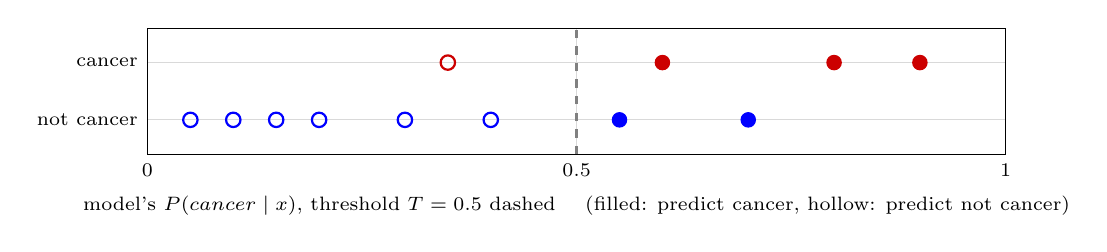
\begin{tikzpicture}
\begin{axis}[scale only axis, width=10.9cm, height=1.6cm,
    xmin=0, xmax=1, ymin=-0.6, ymax=1.6, enlargelimits=false,
    grid=major, grid style={gray!30}, major tick length=0pt,
    xtick={0,0.5,1}, ytick={0,1}, yticklabels={\scriptsize not cancer, \scriptsize cancer},
    xticklabel style={font=\scriptsize},
    xlabel={\scriptsize model's $P(\text{cancer} \mid x)$, threshold $T = 0.5$ dashed \quad (filled: predict cancer, hollow: predict not cancer)}, label style={font=\scriptsize}]
\addplot[gray, dashed, thick] coordinates {(0.5,-0.6) (0.5,1.6)};
% not cancer (t = 0)
\addplot[only marks, mark=o, blue, mark size=2.6pt, thick] coordinates {(0.05,0) (0.10,0) (0.15,0) (0.20,0) (0.30,0) (0.40,0)};
\addplot[only marks, mark=*, blue, mark size=2.6pt] coordinates {(0.55,0) (0.70,0)};
% cancer (t = 1)
\addplot[only marks, mark=o, red!80!black, mark size=2.6pt, thick] coordinates {(0.35,1)};
\addplot[only marks, mark=*, red!80!black, mark size=2.6pt] coordinates {(0.60,1) (0.80,1) (0.90,1)};
\end{axis}
\end{tikzpicture}
\par}
\end{keeptogether}

\subsection*{The Confusion Matrix}
\begin{keeptogether}
Every prediction lands in one of four boxes. ``Positive'' means a prediction of cancer, and ``true'' means the prediction is correct. Counting the tumors above:

{\centering
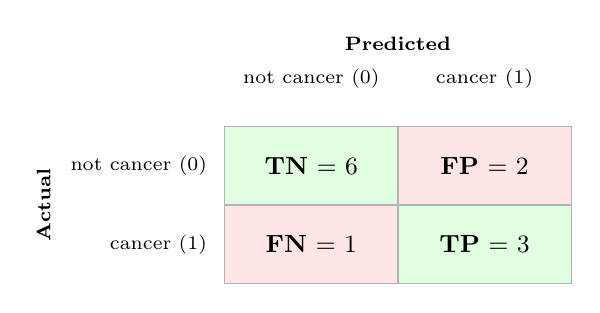
\begin{tikzpicture}[cell/.style={draw=gray!60, minimum width=2.2cm, minimum height=1.0cm, align=center, font=\small}]
\node[font=\scriptsize\bfseries] at (2.2,1.55) {Predicted};
\node[font=\scriptsize] at (1.1,1.1) {not cancer (0)};
\node[font=\scriptsize] at (3.3,1.1) {cancer (1)};
\node[font=\scriptsize\bfseries, rotate=90] at (-2.3,-0.5) {Actual};
\node[font=\scriptsize, anchor=east] at (-0.1,0.0) {not cancer (0)};
\node[font=\scriptsize, anchor=east] at (-0.1,-1.0) {cancer (1)};
\node[cell, fill=green!12] at (1.1,0.0) {\textbf{TN} = 6};
\node[cell, fill=red!10] at (3.3,0.0) {\textbf{FP} = 2};
\node[cell, fill=red!10] at (1.1,-1.0) {\textbf{FN} = 1};
\node[cell, fill=green!12] at (3.3,-1.0) {\textbf{TP} = 3};
\end{tikzpicture}
\par}
{\centering\scriptsize A false positive flags a healthy tumor; a false negative misses a cancer.\par}
\end{keeptogether}

\subsection*{Accuracy, Precision, and Recall}
\begin{keeptogether}
Each metric divides the shaded green cells by all shaded cells:

{\centering
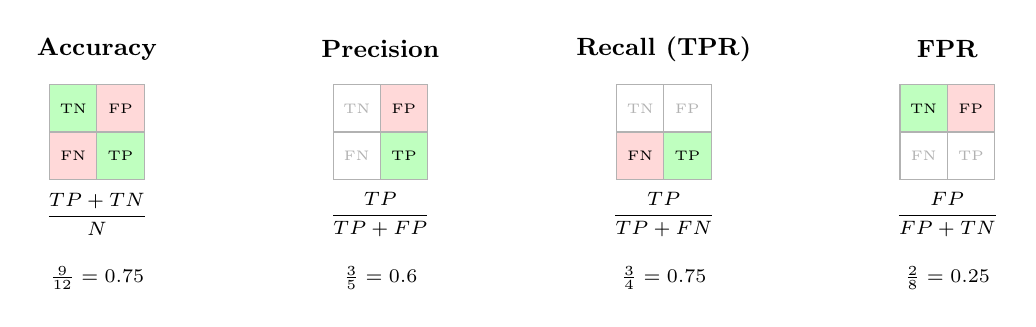
\begin{tikzpicture}[c/.style={draw=gray!60, minimum size=0.6cm, inner sep=0pt, font=\tiny}]
\foreach \px/\name/\tn/\fp/\fn/\tp/\formula/\val in {
    0/Accuracy/g/u/u/g/{\frac{TP + TN}{N}}/{\frac{9}{12} = 0.75},
    3.6/Precision/n/u/n/g/{\frac{TP}{TP + FP}}/{\frac{3}{5} = 0.6},
    7.2/Recall (TPR)/n/n/u/g/{\frac{TP}{TP + FN}}/{\frac{3}{4} = 0.75},
    10.8/FPR/g/u/n/n/{\frac{FP}{FP + TN}}/{\frac{2}{8} = 0.25}} {
  \begin{scope}[shift={(\px,0)}]
  \node[font=\small\bfseries] at (0.3,1.05) {\name};
  \foreach \x/\y/\lab/\s in {0/0.3/TN/\tn, 0.6/0.3/FP/\fp, 0/-0.3/FN/\fn, 0.6/-0.3/TP/\tp} {
    \if\s g \node[c, fill=green!25] at (\x,\y) {\lab};\fi
    \if\s u \node[c, fill=red!15] at (\x,\y) {\lab};\fi
    \if\s n \node[c, text=gray!60] at (\x,\y) {\lab};\fi
  }
  \node[font=\scriptsize] at (0.3,-1.05) {$\displaystyle\formula$};
  \node[font=\scriptsize] at (0.3,-1.85) {$\val$};
  \end{scope}
}
\end{tikzpicture}
\par}
{\centering\scriptsize Green: counted on top. Green + red: counted on the bottom. Gray: not used.\par}
\end{keeptogether}

\begin{keeptogether}
Each metric answers a different question about the tumors:
\begin{itemize}
  \item \textbf{Accuracy:} what fraction of all tumors were classified correctly?
  \item \textbf{Precision:} of the tumors we flagged as cancer, what fraction really are cancer? It penalizes false positives.
  \item \textbf{Recall} (true positive rate, TPR): of the real cancers, what fraction did we catch? It penalizes false negatives.
  \item \textbf{False positive rate} (FPR): of the healthy tumors, what fraction did we wrongly flag?
\end{itemize}
\end{keeptogether}

\subsection*{Why Accuracy Can Mislead}
With \textbf{class imbalance}, accuracy rewards ignoring the rare class. Out of 100 tumors with 5 cancers, a model that always predicts ``not cancer'' gets $\tfrac{95}{100} = 95\%$ accuracy but recall $\tfrac{0}{5} = 0$: it never finds a single cancer. Precision and recall expose this, so they are preferred when one class is rare.

\subsection*{Changing the Threshold}
\begin{keeptogether}
The confusion matrix depends on $T$. Lowering $T$ flags more tumors, so it catches more cancers but also flags more healthy ones:

{\centering
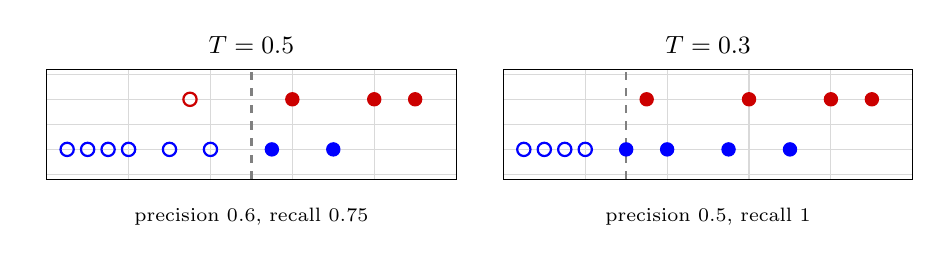
\begin{tikzpicture}
\begin{axis}[name=a,  scale only axis, width=5.2cm, height=1.4cm,
    xmin=0, xmax=1, ymin=-0.6, ymax=1.6, enlargelimits=false,
    grid=major, grid style={gray!30}, major tick length=0pt,
    xticklabels={}, yticklabels={},
    title={\small\textbf{$T = 0.5$}}, title style={yshift=-4pt},
    xlabel={\scriptsize precision $0.6$, recall $0.75$}, label style={font=\scriptsize}]
\addplot[gray, dashed, thick] coordinates {(0.5,-0.6) (0.5,1.6)};
\addplot[only marks, mark=*, blue, mark size=2.4pt] coordinates {(0.55,0) (0.7,0)};
\addplot[only marks, mark=o, blue, thick, mark size=2.4pt] coordinates {(0.05,0) (0.1,0) (0.15,0) (0.2,0) (0.3,0) (0.4,0)};
\addplot[only marks, mark=*, red!80!black, mark size=2.4pt] coordinates {(0.6,1) (0.8,1) (0.9,1)};
\addplot[only marks, mark=o, red!80!black, thick, mark size=2.4pt] coordinates {(0.35,1)};
\end{axis}
\begin{axis}[name=b, at={(a.east)}, anchor=west, xshift=0.6cm, scale only axis, width=5.2cm, height=1.4cm,
    xmin=0, xmax=1, ymin=-0.6, ymax=1.6, enlargelimits=false,
    grid=major, grid style={gray!30}, major tick length=0pt,
    xticklabels={}, yticklabels={},
    title={\small\textbf{$T = 0.3$}}, title style={yshift=-4pt},
    xlabel={\scriptsize precision $0.5$, recall $1$}, label style={font=\scriptsize}]
\addplot[gray, dashed, thick] coordinates {(0.3,-0.6) (0.3,1.6)};
\addplot[only marks, mark=*, blue, mark size=2.4pt] coordinates {(0.3,0) (0.4,0) (0.55,0) (0.7,0)};
\addplot[only marks, mark=o, blue, thick, mark size=2.4pt] coordinates {(0.05,0) (0.1,0) (0.15,0) (0.2,0)};
\addplot[only marks, mark=*, red!80!black, mark size=2.4pt] coordinates {(0.35,1) (0.6,1) (0.8,1) (0.9,1)};
\end{axis}
\end{tikzpicture}
\par}
{\centering\scriptsize Lowering $T$ to 0.3 catches the missed cancer (0.35) but flags two more healthy tumors (0.30, 0.40).\par}
\end{keeptogether}

\begin{keeptogether}
So precision and recall trade off against each other. The \textbf{F1 score} combines them into one number (their harmonic mean), and we can pick the threshold that maximizes it:
\[
F_1 = \frac{2 \cdot \text{precision} \cdot \text{recall}}{\text{precision} + \text{recall}}
\qquad T = 0.5\text{:} \quad \frac{2(0.6)(0.75)}{0.6 + 0.75} = 0.67
\]
\end{keeptogether}

\subsection*{Choosing the Threshold from Error Costs}
\begin{keeptogether}
Missing a cancer is worse than a false alarm. Let $L_{FN}$ and $L_{FP}$ be the cost of each mistake and $p = P(\text{cancer} \mid x)$. Predicting ``not cancer'' risks a miss with probability $p$; predicting ``cancer'' risks a false alarm with probability $1 - p$. We pick the cheaper action:

{\centering
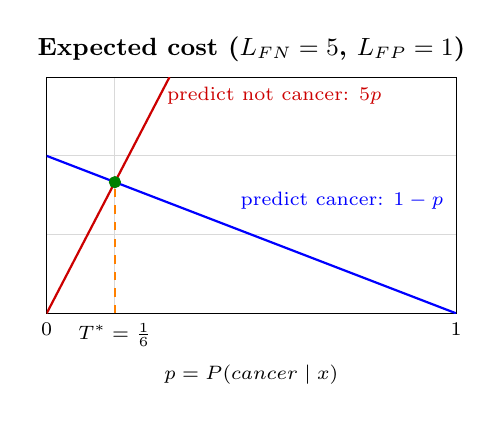
\begin{tikzpicture}
\begin{axis}[scale only axis, width=5.2cm, height=3cm,
    xmin=0, xmax=1, ymin=0, ymax=1.5, enlargelimits=false,
    grid=major, grid style={gray!30}, major tick length=0pt,
    xtick={0,0.1667,1}, xticklabels={\scriptsize 0, \scriptsize $T^* = \frac{1}{6}$, \scriptsize 1}, yticklabels={},
    title={\small\textbf{Expected cost ($L_{FN} = 5$, $L_{FP} = 1$)}}, title style={yshift=-4pt},
    xlabel={\scriptsize $p = P(\text{cancer} \mid x)$}, label style={font=\scriptsize}]
\addplot[thick, red!80!black, domain=0:0.3] {5*x};
\node[font=\scriptsize, red!80!black, anchor=west] at (axis cs:0.27,1.38) {predict not cancer: $5p$};
\addplot[thick, blue, domain=0:1] {1-x};
\node[font=\scriptsize, blue, anchor=south west] at (axis cs:0.45,0.6) {predict cancer: $1 - p$};
\addplot[orange, dashed, thick] coordinates {(0.1667,0) (0.1667,0.833)};
\addplot[only marks, mark=*, green!50!black, mark size=2pt] coordinates {(0.1667,0.833)};
\end{axis}
\end{tikzpicture}
\par}
{\centering\scriptsize Above $T^*$, predicting cancer is the cheaper action.\par}
\end{keeptogether}

\begin{keeptogether}
Setting the two costs equal, $L_{FN}\,p = L_{FP}(1 - p)$, gives the optimal threshold:
\[
T^* = \frac{L_{FP}}{L_{FP} + L_{FN}} \qquad \text{tumors:} \quad \frac{1}{1 + 5} = 0.17
\]
Only the threshold moves; the model does not need to be retrained. With equal costs, $T^* = 0.5$.
\end{keeptogether}

\subsection*{The ROC Curve}
\begin{keeptogether}
The \textbf{ROC curve} plots TPR against FPR for every threshold. Sweeping $T$ from 1 down to 0 moves from the bottom-left corner (nothing flagged) to the top-right corner (everything flagged):

{\centering
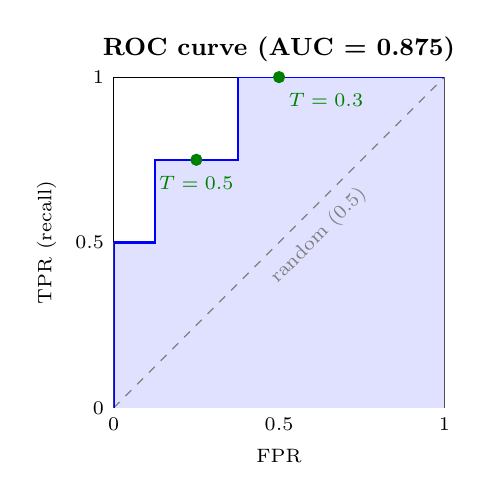
\begin{tikzpicture}
\begin{axis}[scale only axis, width=4.2cm, height=4.2cm,
    xmin=0, xmax=1, ymin=0, ymax=1, enlargelimits=false,
    grid=major, grid style={gray!30}, major tick length=0pt,
    xtick={0,0.5,1}, ytick={0,0.5,1}, ticklabel style={font=\scriptsize},
    title={\small\textbf{ROC curve (AUC = 0.875)}}, title style={yshift=-4pt},
    xlabel={\scriptsize FPR}, ylabel={\scriptsize TPR (recall)}, label style={font=\scriptsize}]
\addplot[fill=blue!12, draw=none] coordinates {(0,0) (0,0.5) (0.125,0.5) (0.125,0.75) (0.375,0.75) (0.375,1) (1,1) (1,0)} \closedcycle;
\addplot[gray, dashed] coordinates {(0,0) (1,1)};
\node[font=\scriptsize, gray, rotate=45] at (axis cs:0.62,0.52) {random (0.5)};
\addplot[thick, blue] coordinates {(0,0) (0,0.5) (0.125,0.5) (0.125,0.75) (0.375,0.75) (0.375,1) (1,1)};
\addplot[only marks, mark=*, green!50!black, mark size=2pt] coordinates {(0.25,0.75) (0.5,1)};
\node[font=\scriptsize, green!50!black, anchor=north] at (axis cs:0.25,0.73) {$T = 0.5$};
\node[font=\scriptsize, green!50!black, anchor=north west] at (axis cs:0.5,0.98) {$T = 0.3$};
\end{axis}
\end{tikzpicture}
\par}
{\centering\scriptsize Shaded: the area under the curve (AUC).\par}
\end{keeptogether}

\begin{keeptogether}
A good classifier hugs the top-left corner (high TPR, low FPR). The \textbf{area under the curve} (AUC) summarizes this in one number:
\begin{itemize}
  \item \textbf{AUC = 1:} perfect; some threshold separates the classes completely.
  \item \textbf{AUC = 0.5:} random guessing (the diagonal).
  \item \textbf{AUC below 0.5:} worse than random.
\end{itemize}
\end{keeptogether}

\subsection*{More Than Two Classes}
\begin{keeptogether}
With $K > 2$ classes, the model outputs one score $a_k$ per class, and the \textbf{softmax} turns the scores into probabilities that sum to 1:
\[
P(C_k \mid \mathbf{x}) = \frac{e^{a_k}}{\sum_{j=1}^{K} e^{a_j}}
\qquad \text{scores } (2, 1, 0) \;\Rightarrow\; (0.67,\ 0.24,\ 0.09)
\]
We predict the class with the highest probability. For $K = 2$, softmax reduces to the sigmoid. Two older alternatives combine binary classifiers instead:
\begin{itemize}
  \item \textbf{One-versus-rest:} one classifier per class, separating it from all the others.
  \item \textbf{One-versus-one:} one classifier per pair of classes, $\tfrac{K(K-1)}{2}$ in total.
\end{itemize}
\end{keeptogether}
